\documentclass[notheorems]{beamer}

%packages
\usepackage[utf8]{inputenc}
\usepackage[english]{babel}
\usepackage{float}
\usepackage{tikz}
\usepackage{pgfplots}
\usepackage{geometry}
\usepackage{amsfonts, amssymb, amsmath}             % Fonte e símbolos matemáticos
%\usepackage[english,ruled,lined,linesnumbered]{algorithm2e}    % Escrever algoritmos
\usepackage{algorithm,algorithmic}
\usepackage{amsthm}
\usepackage{theoremref}
\usepackage[autostyle]{csquotes}
\usepackage{multicol}
\usepackage{biblatex}
%biber latex settings
\addbibresource{mybib.bib}

\usepackage[utf8]{inputenc}

\addtobeamertemplate{navigation symbols}{}{%
  \usebeamerfont{footline}%
  \usebeamercolor[fg]{footline}%
  \hspace{1em}%
  \insertframenumber/\inserttotalframenumber
}
\setbeamercolor{footline}{fg=blue}
\setbeamerfont{footline}{series=\bfseries}

\makeatletter
\newtheorem{problem}{\translate{Problem}}
\newtheorem{solution}{\translate{Solution}}

\theoremstyle{definition}
\newtheorem{definition}{\translate{Definition}}
\newtheorem{definitions}{\translate{Definitions}}

\theoremstyle{example}
\newtheorem{example}{\translate{Example}}
\newtheorem{examples}{\translate{Examples}}

% Compatibility
\newtheorem{Beispiel}{Beispiel}
\newtheorem{Beispiele}{Beispiele}
\theoremstyle{plain}
\newtheorem{Loesung}{L\"osung}
\newtheorem{Satz}{Satz}
\newtheorem{Folgerung}{Folgerung}
\newtheorem{Fakt}{Fakt}
\newenvironment{Proof}{\begin{proof}}{\end{proof}}
\newenvironment{Problem}{\begin{problem}}{\end{problem}}
\newenvironment{Example}{\begin{example}}{\end{example}}
\newenvironment{Examples}{\begin{examples}}{\end{examples}}
\newenvironment{Definition}{\begin{definition}}{\end{definition}}
\newenvironment{claim}[1]{\par\noindent\blue{Claim:}\space#1}{}
\newenvironment{claimproof}[1]{\par\noindent\blue{Proof:}\space#1}{\hfill $\blacksquare$}
\makeatother

%tikz settings
\usetikzlibrary{arrows,positioning,automata,shadows,fit,shapes,calc,shapes.geometric}
\tikzset{triangle_black/.style={regular polygon, regular polygon sides=3, minimum size=0.3cm, fill=black}}
\tikzset{triangle/.style={regular polygon, regular polygon sides=3, minimum size=0.3cm, fill=white}}
\tikzset{square/.style={regular polygon, regular polygon sides=4, minimum size=0.3cm, fill=white}}
\tikzset{circufe/.style={circle,draw, minimum size=0.2cm, fill=white}}
\tikzset{raio/.style={circle,draw, minimum size=1.45cm, fill=white}} 
\tikzset{circle_new/.style={circle,draw, minimum size=0.2cm, fill=white}}   
\tikzset{label/.style={draw=black, fill=white}}   

\newcounter{savedenum}
\newcommand*{\saveenum}{\setcounter{savedenum}{\theenumi}}
\newcommand*{\resume}{\setcounter{enumi}{\thesavedenum}}
\newcommand{\blue}[1]{\textcolor{blue}{#1}}

%Information to be included in the title page:
\title{Elementary Resource Constrained Shortest Path Problem (ERCSPP)}
\author{Matheus Diógenes Andrade\\
\href{mailto:matheusdiogenesandrade@gmail.com}{matheusdiogenesandrade@gmail.com}\\
Fábio Luiz Usberti\\
\href{mailto:fusberti@ic.unicamp.br}{fusberti@ic.unicamp.br}\\
Rafael Kendy Arakaki\\
\href{mailto:rafaelkendyarakaki@gmail.com}{rafaelkendyarakaki@gmail.com}
}
\institute{Institute of Computing - University of Campinas}
\date{2021}

\begin{document}

\frame{\titlepage}

\begin{frame}
  \frametitle{Topics}
  Presentation based on \footfullcite{FeilletDejaxGendreauGueguen2004}.
  \begin{enumerate}
    \item Problem definition;
    \item Properties;
    \item Algorithm;
  \end{enumerate}
\end{frame}

\begin{frame}
  \begin{center}
    \Huge Problem definition
  \end{center}
\end{frame}

\begin{frame}
  \frametitle{Problem definition}
  Let
  \begin{itemize}
    \item \blue{$D(V = \{s\} \cup V^{+} \cup \{t\}, A)$} be the digraph, where
    \begin{itemize}
      \item \blue{$s$} is the source node; and 
      \item \blue{$t$} is the target node.
    \end{itemize}
    \item \blue{$c_a \in \mathbb{R}$} be the arc \blue{$a \in A$} cost;
    \item \blue{$R$} be the set of resources;
    \item \blue{$d^r_a \in \mathbb{R}$} be the metric resource \blue{$r \in R$} consumption of the arc \blue{$a \in A$};
    \item \blue{$w^r_i = [b^r_i, e^r_i]$} be the resource \blue{$r \in R$} window of the node \blue{$i \in V$}.
  \end{itemize}
\end{frame}

\begin{frame}
  \frametitle{Problem definition}
  Let
  \begin{itemize}
    \item \blue{$P$} be an elementary resource constrained \blue{$s$}-\blue{$t$}-path in \blue{$D$}; and
    \item \blue{$S_i^r$} be the resource \blue{$r \in R$} consumption of node \blue{$i \in V(P)$},
  such that \blue{$\forall (i, j) \in A(P) (\forall r \in R (S_j^r = \text{max} \{S_i^r + d_{ij}^r, b_j^r\} \leqslant e_j^r))$}.
  \end{itemize}
  The ERCSPP consists in finding the shortest elementary resource constrained \blue{$s$}-\blue{$t$}-path \blue{$P$} in \blue{$D$}.
\end{frame}

\begin{frame}
  \frametitle{Problem definition}
  \blue{$c_a: (d^1_a, d^2_a)$}
  \begin{figure}[H]
    \centering
    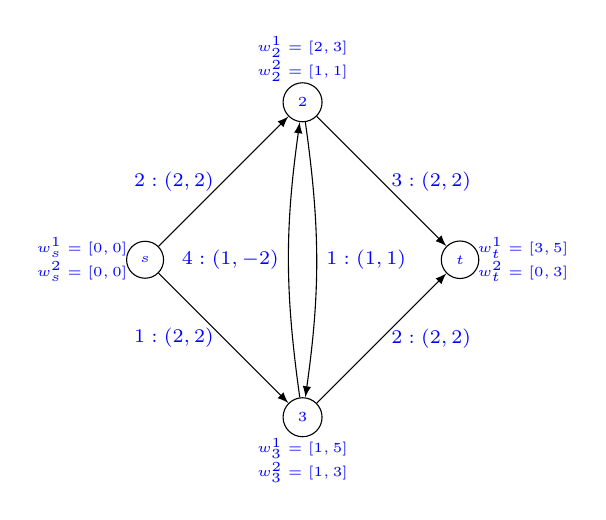
\begin{tikzpicture}[font=\tiny]
      %nodes
      \node at (-0.8, 0.15) {\blue{$w_s^1 = [0,0]$}};
      \node at (-0.8, -0.15) {\blue{$w_s^2 = [0,0]$}};
      \node[circle, draw] (s) at (0, 0) {\blue{$s$}};
      \node at (2, 2.7) {\blue{$w_2^1 = [2, 3]$}};
      \node at (2, 2.4) {\blue{$w_2^2 = [1, 1]$}};
      \node[circle, draw] (a) at (2, 2) {\blue{$2$}};
      \node at (2, -2.4) {\blue{$w_3^1 = [1, 5]$}};
      \node at (2, -2.7) {\blue{$w_3^2 = [1, 3]$}};
      \node[circle, draw] (b) at (2, -2) {\blue{$3$}};
      \node at (4.8, 0.15) {\blue{$w_t^1 = [3, 5]$}};
      \node at (4.8, -0.15) {\blue{$w_t^2 = [0, 3]$}};
      \node[circle, draw] (t) at (4, 0) {\blue{$t$}};
      %edges
      \path [draw,-latex] (s) to node[left]{\scriptsize\blue{$2: (2, 2)$}} (a);
      \path [draw,-latex] (s) to node[left]{\scriptsize\blue{$1: (2, 2)$}} (b);
      \path [draw,-latex] (a) to node[right]{\scriptsize\blue{$3: (2, 2)$}} (t);
      \path [draw,-latex] (b) to node[right]{\scriptsize\blue{$2: (2, 2)$}} (t);
      \path [draw,-latex] (a) edge [bend left=8] node[right]{\scriptsize\blue{$1: (1, 1)$}} (b);
      \path [draw,-latex] (b) edge [bend left=8] node[left]{\scriptsize\blue{$4: (1, -2)$}} (a);
    \end{tikzpicture}
    \caption{A ERCSPP instance digraph example.}
  \end{figure}
\end{frame}

\begin{frame}
  \frametitle{Problem definition}
  \blue{$c_a: (d^1_a, d^2_a)$}
  \begin{figure}[H]
    \centering
    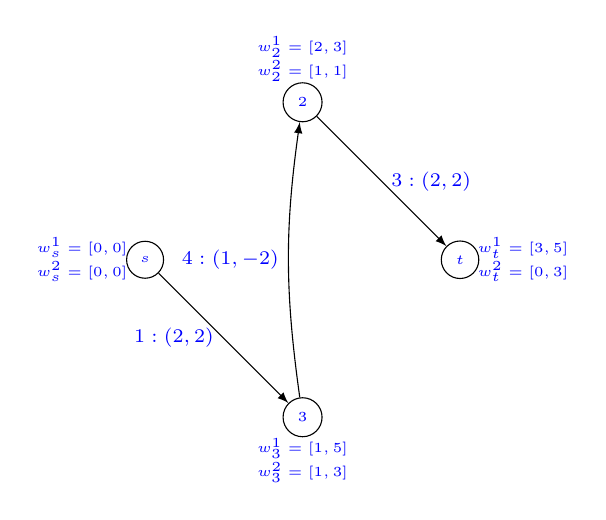
\begin{tikzpicture}[font=\tiny]
      %nodes
      \node at (-0.8, 0.15) {\blue{$w_s^1 = [0,0]$}};
      \node at (-0.8, -0.15) {\blue{$w_s^2 = [0,0]$}};
      \node[circle, draw] (s) at (0, 0) {\blue{$s$}};
      \node at (2, 2.7) {\blue{$w_2^1 = [2, 3]$}};
      \node at (2, 2.4) {\blue{$w_2^2 = [1, 1]$}};
      \node[circle, draw] (a) at (2, 2) {\blue{$2$}};
      \node at (2, -2.4) {\blue{$w_3^1 = [1, 5]$}};
      \node at (2, -2.7) {\blue{$w_3^2 = [1, 3]$}};
      \node[circle, draw] (b) at (2, -2) {\blue{$3$}};
      \node at (4.8, 0.15) {\blue{$w_t^1 = [3, 5]$}};
      \node at (4.8, -0.15) {\blue{$w_t^2 = [0, 3]$}};
      \node[circle, draw] (t) at (4, 0) {\blue{$t$}};
      %edges
      \path [draw,-latex] (s) to node[left]{\scriptsize\blue{$1: (2, 2)$}} (b);
      \path [draw,-latex] (b) edge [bend left=8] node[left]{\scriptsize\blue{$4: (1, -2)$}} (a);
      \path [draw,-latex] (a) to node[right]{\scriptsize\blue{$3: (2, 2)$}} (t);
    \end{tikzpicture}
    \caption{The solution of the previous instance.}
  \end{figure}
\end{frame}


\begin{frame}
  \begin{center}
    \Huge Properties
  \end{center}
\end{frame}

\begin{frame}
  \frametitle{Properties}
  \framesubtitle{Node state/label I}
  Let
  \begin{itemize}
    \item \blue{$P_i$} be an elementary path from \blue{$s$} to \blue{$i \in V$} in \blue{$D$}; and 
    \item \blue{$S_i = (L_i = (l^1_i, ..., l^{|R|}_i), C_i)$} be the state or label of node \blue{$i \in V(P_i)$} in the path \blue{$P_i$}, where:
    \begin{itemize}
      \item \blue{$l^r_i \in \mathbb{R}_{+}$} is the amount of resource \blue{$r \in R$} consumed by the path \blue{$P_i$} at \blue{$i \in V(P_i)$}; and 
      \item \blue{$C_i \in \mathbb{R}$} is the cost of path \blue{$P_i$} at \blue{$i \in V(P_i)$}.
    \end{itemize}
  \end{itemize}
\end{frame}

\begin{frame}
  \frametitle{Properties}
  \framesubtitle{Node state/label I}
  \blue{$P_2, S_3 = (L_3 = (2, 2), 1), S_2 = (L_2 = (3, 0), 5)$}
  \begin{figure}[H]
    \centering
    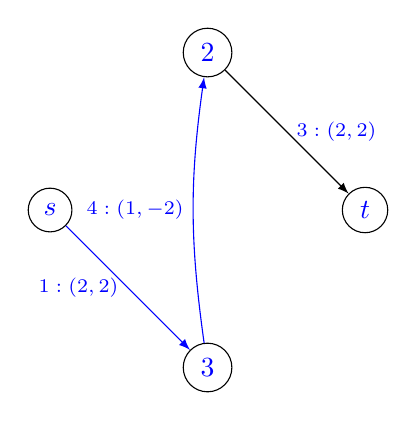
\begin{tikzpicture}
      %nodes
      \node[circle, draw] (s) at (0, 0) {\blue{$s$}};
      \node[circle, draw] (a) at (2, 2) {\blue{$2$}};
      \node[circle, draw] (b) at (2, -2) {\blue{$3$}};
      \node[circle, draw] (t) at (4, 0) {\blue{$t$}};
      %edges
      \path [blue, draw,-latex] (s) to node[left]{\scriptsize\blue{$1: (2, 2)$}} (b);
      \path [blue, draw,-latex] (b) edge [bend left=8] node[left]{\scriptsize\blue{$4: (1, -2)$}} (a);
      \path [draw,-latex] (a) to node[right]{\scriptsize\blue{$3: (2, 2)$}} (t);
    \end{tikzpicture}
    \caption{\blue{$P_2$}.}
    \label{fig:vrptw_disposable_example}
  \end{figure}
\end{frame}

\begin{frame}
  \frametitle{Properties}
  \framesubtitle{Dominance I}
  Let
  \begin{itemize}
    \item \blue{$P_i$} and \blue{$P^{'}_i$} be two distinct elementary paths from \blue{$s$} to \blue{$i \in V$} in \blue{$D$}; and
    \item \blue{$S_i$} and \blue{$S^{'}_i$} be the respective labels.
  \end{itemize}
  \begin{definition}
    \blue{$P_i$} dominates \blue{$P^{'}_i \leftrightarrow S_i \leqslant S^{'}_i$}.
  \end{definition}
\end{frame}

\begin{frame}
  \frametitle{Properties}
  \framesubtitle{Node state/label II}
  Let
  \begin{itemize}
    \item \blue{$L_i = (l^1_i, ..., l^{|R|}_i, s_i, v_i^1, ..., v_i^{|V|})$} be the the  new resources state/label, where:
      \item the number of visited nodes, and the visitation vector by the path \blue{$P_i$}.
    \begin{itemize}
      \item \blue{$l^r_i \in \mathbb{R}_{+}$} is the amount of resource \blue{$r \in R$} consumed by the path \blue{$P_i$} at \blue{$i \in V(P_i)$};
      \item \blue{$s_i = \sum_{j = 1}^{|V|} v_i^j$} is the number of nodes visited by the path \blue{$P_i$} at \blue{$i \in V(P_i)$}; and 
      \item \blue{$v_i^j \in \mathbb{B}$} is equals to \blue{$1$} if node \blue{$j \in V$} is visited by the path \blue{$P_i$} at \blue{$i \in V(P_i)$} and \blue{$0$} otherwise.
    \end{itemize}
  \end{itemize}
\end{frame}

\begin{frame}
  \frametitle{Properties}
  \framesubtitle{Node state/label II}
  \blue{$P_2, S_s = (L_s = (0, 0, 1, 1, 0, 0, 0), 0) , S_3 = (L_3 = (2, 2, 2, 1, 0, 1, 0), 1), S_2 = (L_2 = (3, 0, 3, 1, 1, 1, 0), 5)$}
  \begin{figure}[H]
    \centering
    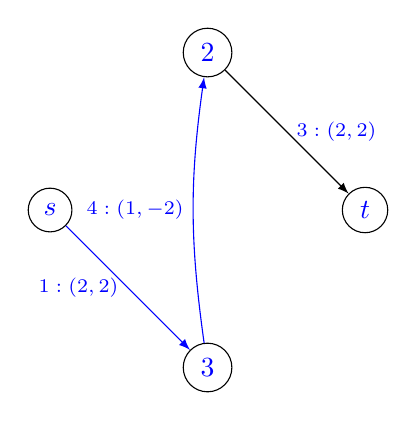
\begin{tikzpicture}
      %nodes
      \node[circle, draw] (s) at (0, 0) {\blue{$s$}};
      \node[circle, draw] (a) at (2, 2) {\blue{$2$}};
      \node[circle, draw] (b) at (2, -2) {\blue{$3$}};
      \node[circle, draw] (t) at (4, 0) {\blue{$t$}};
      %edges
      \path [blue, draw,-latex] (s) to node[left]{\scriptsize\blue{$1: (2, 2)$}} (b);
      \path [blue, draw,-latex] (b) edge [bend left=8] node[left]{\scriptsize\blue{$4: (1, -2)$}} (a);
      \path [draw,-latex] (a) to node[right]{\scriptsize\blue{$3: (2, 2)$}} (t);
    \end{tikzpicture}
    \caption{\blue{$P_2$}.}
    \label{fig:vrptw_disposable_example}
  \end{figure}
\end{frame}

\begin{frame}
  \frametitle{Properties}
  \framesubtitle{Dominance II}
  Let
  \begin{itemize}
    \item \blue{$P_i$} and \blue{$P^{'}_i$} be two distinct elementary paths from \blue{$s$} to \blue{$i \in V$} in \blue{$D$}; and
    \item \blue{$S_i$} and \blue{$S^{'}_i$} be the paths respective labels.
  \end{itemize}
  \begin{definition}
    \blue{$P_i$} dominates \blue{$P^{'}_i \leftrightarrow S_i \leqslant S^{'}_i$}.
  \end{definition}
\end{frame}

\begin{frame}
  \frametitle{Properties}
  \framesubtitle{Unreachable nodes}
  Let
  \begin{itemize}
    \item \blue{$P_i$} be an elementary path from \blue{$s$} to \blue{$i \in V$} in \blue{$D$}; 
    \item \blue{$S_i$} be the path label; and
    \item \blue{$k \in V$} be a digraph node.
  \end{itemize}
  \begin{definition}
    \blue{$k$} is said to be unreachable by \blue{$P_i \rightarrow k \in V(P_i) \vee \exists r \in R (l_i^r + d_{ik}^r > e^r_k)$}.
  \end{definition}
  Note that, does not exist any path from \blue{$i$} that permits to reach it, due to the digraph metricity.
\end{frame}

\begin{frame}
  \frametitle{Properties}
  \framesubtitle{Node state/label III}
  Let
  \begin{itemize}
    \item \blue{$L_i = (l^1_i, ..., l^{|R|}_i, s_i, v_i^1, ..., v_i^{|V|})$} be the the new resources state/label, where:
      \item the number of visited nodes, and the visitation vector by the path \blue{$P_i$}.
    \begin{itemize}
      \item \blue{$l^r_i \in \mathbb{R}_{+}$} is the amount of resource \blue{$r \in R$} consumed by the path \blue{$P_i$} at \blue{$i \in V(P_i)$};
      \item \blue{$s_i = \sum_{j = 1}^{|V|} v_i^j$} is the number of unreachable nodes by the path \blue{$P_i$} at \blue{$i \in V(P_i)$}; and 
      \item \blue{$v_i^j \in \mathbb{B}$} is equals to \blue{$1$} if node \blue{$j \in V$} is unreachable by the path \blue{$P_i$} at \blue{$i \in V(P_i)$} and \blue{$0$} otherwise.
    \end{itemize}
  \end{itemize}
\end{frame}

\begin{frame}
  \frametitle{Properties}
  \framesubtitle{Nondominated paths}
  \begin{claim}
    In order to find the ERCSPP optimal solution, suffices to consider only nondominated paths.
  \end{claim}
  \begin{claimproof}
    Let's consider two elementary paths \blue{$P_i$} and \blue{$P^{'}_i$} from \blue{$s$} to \blue{$i \in V$}, along with its labels \blue{$S_i$} and \blue{$S^{'}_i$}, such that \blue{$P_i$} dominates \blue{$P^{'}_i$}.
    Also, let's consider an arc \blue{$(i, j) \in A : \forall r \in R (l_i^{'r} + d_{ij}^r \leqslant e_j^r) \wedge v_i^{'j} = 0$}.
    Note that \blue{$\forall r \in R (l_i^r + d_{ij}^r \leqslant e_j^r) \wedge v_i^{j} = 0 \wedge C_i \leqslant C^{'}_i$}.
  \end{claimproof}
\end{frame}


\begin{frame}
  \begin{center}
    \Huge Algorithm
  \end{center}
\end{frame}

\begin{frame}
  \frametitle{Algorithm}
  \framesubtitle{Notations I}
  Let
  \begin{itemize}
    \item \blue{$\Lambda_i$} be the list of labels on node \blue{$i \in V$};
    \item \blue{$N$} be the list of nodes to be processed;
    \item \blue{$ E(S_i, j) = (\text{max} \{l^r_i + d_{ij}^r, b^r_j\} : r \in R) \cup (s_i + 1, v_i^1, ..., v_i^j + 1, $} \blue{$..., v_i^{|V|}) $} be the function that returns the label resulting from the extension of a path \blue{$P_i$} by a node \blue{$j$} (\blue{$O(|R|)$});
    \item \blue{\[
        f(S_i, j) =  
        \begin{cases}
          \text{\textcolor{black}{true}},  & \text{\textcolor{black}{if} }      \forall r \in R (\text{max} \{l^r_i + d_{ij}^r, b^r_j\}  \leqslant e_i^r) \wedge \neg v_i^j\\
          \text{\textcolor{black}{false}}, & \text{\textcolor{black}{otherwise}}
        \end{cases}
    \]} be a function that says whether an extension is feasible (\blue{$O(|R|)$});
    \item \blue{$F_{ij}$} be the set of labels extended from \blue{$i$} to \blue{$j \in V$}; and
  \end{itemize}
\end{frame}

\begin{frame}
  \frametitle{Algorithm}
  \framesubtitle{Notations II}
  Let
  \begin{itemize}
    \item \blue{$N_D(\Lambda) = \{S_i \in \Lambda : \nexists S^{'}_i \in \Lambda (S^{'}_i \neq S_i \wedge S^{'}_i \leqslant S_i) \}$} be the function that returns all nondominated labels from \blue{$\Lambda$}. 
      \begin{itemize}
        \item A na\"{i}ve algorithm would take \blue{$O(|\Lambda||R|)$} to check whether a state is nondominated. However, keeping \blue{$|R|$} Binary Seach Trees (BSTs) associated with the labels set \blue{$\Lambda_i$} may help us to reduce the time complexity;
        \item Let \blue{$BST_i^r$} be the BST containing all the resource \blue{$r \in R$} consumptions of all labels in \blue{$\Lambda_i$}, 
              \blue{$g(BST_i^r, l_i^r)$} be the rightmost position of \blue{$BST_i^r$} whose value is equals to or less than \blue{$l_i^r$},
              and \blue{$S(BST_i^{rj})$} be the label associated with the resource consumption at the \blue{$j$}-th position of \blue{$BST_i^r$};
        \item To check if a label \blue{$S_i$} is nondominated it would take \blue{$O(\textcolor{black}{min}_{r \in R} \{ g(BST_i^r, l_i^r) \} |R| + |R|\textcolor{black}{log}_2^{|R|})$};
        \item Note that the above complexity may be worst than the na\"{i}ve one, when \blue{$\textcolor{black}{min}_{r \in R} \{ g(BST_i^r, l_i^r) \} = |\Lambda_i|$};
        \item But even though such case may not be so frequent, and besides that choosing the threshold \blue{$\textcolor{black}{min}_{r \in R} \{ g(BST_i^r, l_i^r) \} \leqslant |\Lambda_i|$} can be a good choice, since \blue{$|\Lambda_i|$} grows exponentially.
      \end{itemize}
  \end{itemize}
\end{frame}

\begin{frame}
  \frametitle{Algorithm}
  \framesubtitle{Code}
  \begin{algorithm}[H]
    \scriptsize
    \begin{algorithmic}[1]
      \REQUIRE \blue{$D(V, A), c_a \quad \forall a \in A, d_a^r \quad \forall a \in A, r \in R$}
      %initialization
      \STATE \blue{$\Lambda_s \gets \{ (\{0\}^{|R|} \cup (1, 1) \cup \{0\}^{|V| - 1}, 0) \}$};
      \STATE \blue{$\Lambda_i \gets \emptyset \quad \forall i \in V \backslash \{s\}$};
      \STATE \blue{$N \gets \{s\}$};
      %exploration
      \label{algo1:setp:main_while}\WHILE {\blue{$N \neq \emptyset$}}
        \STATE Let \blue{$i \in N$} be a \blue{$N$} arbitrary node;
        \label{algo1:setp:explore_arcs}\FORALL {\blue{$(i, j) \in \delta^{+}(i)$}}
          \STATE \blue{$F_{ij} \gets \emptyset$};
          \FORALL {\blue{$S_i \in \Lambda_i$}}
            \IF {\blue{$f(S_i, j)$}}
              \STATE \blue{$F_{ij} \gets F_{ij} \cup \{E(S_i, j)\}$};
            \ENDIF
          \ENDFOR
          \STATE \blue{$\Lambda_j \gets N_D(F_{ij} \cup \Lambda_j)$};
          \IF {\blue{$\Lambda_j$} has changed}
            \STATE \blue{$N \gets N \cup \{j\}$};
          \ENDIF
        \ENDFOR
        \STATE \blue{$N \gets N \backslash \{i\}$};
      \ENDWHILE
      \RETURN \blue{min$_{(L_t, C_t) \in \Lambda_t} \{ C_t \}$} if \blue{$\Lambda_t \neq \emptyset$} else \blue{$\infty$};
    \end{algorithmic}
    \caption{Labeling algorithm}
    \label{alg:seq}
  \end{algorithm}
\end{frame}

\begin{frame}
  \frametitle{Algorithm}
  \framesubtitle{Example}
  \begin{multicols}{2}
    State before line \ref{algo1:setp:main_while}:
    \begin{itemize}   
      \item \blue{$\Lambda_s = \{ ((0, 0, 1, 1, 0, 0, 0), 0) \}$};
      \item \blue{$\Lambda_2 = \Lambda_3 = \Lambda_t = \emptyset$};
      \item \blue{$N = \{\{s\}\}$};
    \end{itemize}   
    \begin{figure}[H]
      \centering
      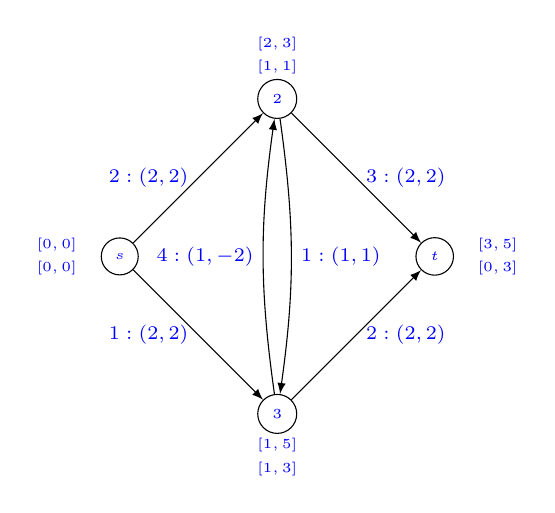
\begin{tikzpicture}[font=\tiny]
        %nodes
        \node at (-0.8, 0.15) {\blue{$[0,0]$}};
        \node at (-0.8, -0.15) {\blue{$[0,0]$}};
        \node[circle, draw] (s) at (0, 0) {\blue{$s$}};
        \node at (2, 2.7) {\blue{$[2, 3]$}};
        \node at (2, 2.4) {\blue{$[1, 1]$}};
        \node[circle, draw] (a) at (2, 2) {\blue{$2$}};
        \node at (2, -2.4) {\blue{$[1, 5]$}};
        \node at (2, -2.7) {\blue{$[1, 3]$}};
        \node[circle, draw] (b) at (2, -2) {\blue{$3$}};
        \node at (4.8, 0.15) {\blue{$[3, 5]$}};
        \node at (4.8, -0.15) {\blue{$[0, 3]$}};
        \node[circle, draw] (t) at (4, 0) {\blue{$t$}};
        %edges
        \path [draw,-latex] (s) to node[left]{\scriptsize\blue{$2: (2, 2)$}} (a);
        \path [draw,-latex] (s) to node[left]{\scriptsize\blue{$1: (2, 2)$}} (b);
        \path [draw,-latex] (a) to node[right]{\scriptsize\blue{$3: (2, 2)$}} (t);
        \path [draw,-latex] (b) to node[right]{\scriptsize\blue{$2: (2, 2)$}} (t);
        \path [draw,-latex] (a) edge [bend left=8] node[right]{\scriptsize\blue{$1: (1, 1)$}} (b);
        \path [draw,-latex] (b) edge [bend left=8] node[left]{\scriptsize\blue{$4: (1, -2)$}} (a);
      \end{tikzpicture}
      \caption{A ERCSPP instance digraph example.}
    \end{figure}
  \end{multicols}
\end{frame}

\begin{frame}
  \frametitle{Algorithm}
  \framesubtitle{Example}
  \begin{multicols}{2}
    State at the end of \blue{$1$}st iteration of the while at line \ref{algo1:setp:main_while}:
    \begin{itemize}   
      \item \blue{$\Lambda_s = \{ ((0, 0, 1, 1, 0, 0, 0), 0) \}$};
      \item \blue{$\Lambda_2 = \emptyset$};
      \item \blue{$\Lambda_3 = \{((2, 2, 2, 1, 0, 1, 0), 1)\}$};
      \item \blue{$\Lambda_t = \emptyset$};
      \item \blue{$N = \{\{3\}\}$};
    \end{itemize}   
    \begin{figure}[H]
      \centering
      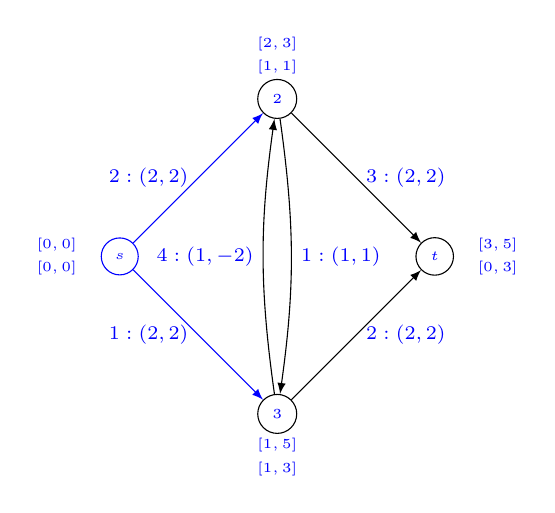
\begin{tikzpicture}[font=\tiny]
        %nodes
        \node at (-0.8, 0.15) {\blue{$[0,0]$}};
        \node at (-0.8, -0.15) {\blue{$[0,0]$}};
        \node[blue, circle, draw] (s) at (0, 0) {\blue{$s$}};
        \node at (2, 2.7) {\blue{$[2, 3]$}};
        \node at (2, 2.4) {\blue{$[1, 1]$}};
        \node[circle, draw] (a) at (2, 2) {\blue{$2$}};
        \node at (2, -2.4) {\blue{$[1, 5]$}};
        \node at (2, -2.7) {\blue{$[1, 3]$}};
        \node[circle, draw] (b) at (2, -2) {\blue{$3$}};
        \node at (4.8, 0.15) {\blue{$[3, 5]$}};
        \node at (4.8, -0.15) {\blue{$[0, 3]$}};
        \node[circle, draw] (t) at (4, 0) {\blue{$t$}};
        %edges
        \path [blue, draw,-latex] (s) to node[left]{\scriptsize\blue{$2: (2, 2)$}} (a);
        \path [blue, draw,-latex] (s) to node[left]{\scriptsize\blue{$1: (2, 2)$}} (b);
        \path [draw,-latex] (a) to node[right]{\scriptsize\blue{$3: (2, 2)$}} (t);
        \path [draw,-latex] (b) to node[right]{\scriptsize\blue{$2: (2, 2)$}} (t);
        \path [draw,-latex] (a) edge [bend left=8] node[right]{\scriptsize\blue{$1: (1, 1)$}} (b);
        \path [draw,-latex] (b) edge [bend left=8] node[left]{\scriptsize\blue{$4: (1, -2)$}} (a);
      \end{tikzpicture}
      \caption{Arcs explored the for loop at line \ref{algo1:setp:explore_arcs} when \blue{$i = s$}.}
    \end{figure}
  \end{multicols}
\end{frame}

\begin{frame}
  \frametitle{Algorithm}
  \framesubtitle{Example}
  \begin{multicols}{2}
    State at the end of \blue{$2$}rd iteration of the while at line \ref{algo1:setp:main_while}:
    \begin{itemize}   
      \item \blue{$\Lambda_s = \{ ((0, 0, 1, 1, 0, 0, 0), 0) \}$};
      \item \blue{$\Lambda_2 = \{((3, 0, 3, 1, 1, 1, 0), 5)\}$};
      \item \blue{$\Lambda_3 = \{((2, 2, 2, 1, 0, 1, 0), 1)\}$};
      \item \blue{$\Lambda_t = \emptyset$};
      \item \blue{$N = \{\{2\}\}$};
    \end{itemize}   
    \begin{figure}[H]
      \centering
      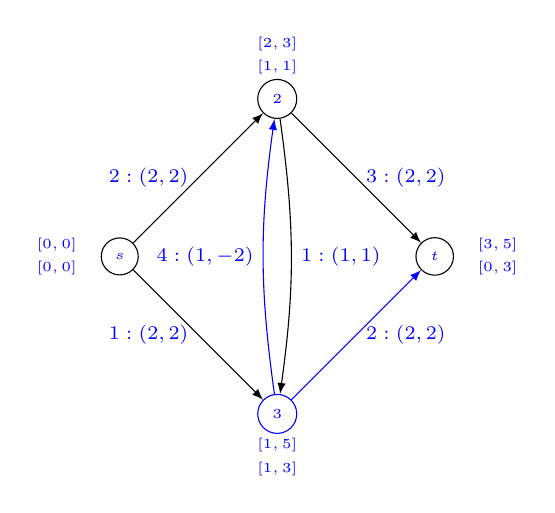
\begin{tikzpicture}[font=\tiny]
        %nodes
        \node at (-0.8, 0.15) {\blue{$[0,0]$}};
        \node at (-0.8, -0.15) {\blue{$[0,0]$}};
        \node[circle, draw] (s) at (0, 0) {\blue{$s$}};
        \node at (2, 2.7) {\blue{$[2, 3]$}};
        \node at (2, 2.4) {\blue{$[1, 1]$}};
        \node[circle, draw] (a) at (2, 2) {\blue{$2$}};
        \node at (2, -2.4) {\blue{$[1, 5]$}};
        \node at (2, -2.7) {\blue{$[1, 3]$}};
        \node[blue, circle, draw] (b) at (2, -2) {\blue{$3$}};
        \node at (4.8, 0.15) {\blue{$[3, 5]$}};
        \node at (4.8, -0.15) {\blue{$[0, 3]$}};
        \node[circle, draw] (t) at (4, 0) {\blue{$t$}};
        %edges
        \path [draw,-latex] (s) to node[left]{\scriptsize\blue{$2: (2, 2)$}} (a);
        \path [draw,-latex] (s) to node[left]{\scriptsize\blue{$1: (2, 2)$}} (b);
        \path [draw,-latex] (a) to node[right]{\scriptsize\blue{$3: (2, 2)$}} (t);
        \path [blue, draw,-latex] (b) to node[right]{\scriptsize\blue{$2: (2, 2)$}} (t);
        \path [draw,-latex] (a) edge [bend left=8] node[right]{\scriptsize\blue{$1: (1, 1)$}} (b);
        \path [blue, draw,-latex] (b) edge [bend left=8] node[left]{\scriptsize\blue{$4: (1, -2)$}} (a);
      \end{tikzpicture}
      \caption{Arcs explored the for loop at line \ref{algo1:setp:explore_arcs} when \blue{$i = 3$}.}
    \end{figure}
  \end{multicols}
\end{frame}

\begin{frame}
  \frametitle{Algorithm}
  \framesubtitle{Example}
  \begin{multicols}{2}
    State at the end of \blue{$3$}nd iteration of the while at line \ref{algo1:setp:main_while}:
    \begin{itemize}   
      \item \blue{$\Lambda_s = \{ ((0, 0, 1, 1, 0, 0, 0), 0) \}$};
      \item \blue{$\Lambda_2 = \{((3, 0, 3, 1, 1, 1, 0), 5)\}$};
      \item \blue{$\Lambda_3 = \{((2, 2, 2, 1, 0, 1, 0), 1)\}$};
      \item \blue{$\Lambda_t = \{((5, 2, 4, 1, 1, 1, 1), 8)\}$};
      \item \blue{$N = \{\{t\}\}$};
    \end{itemize}   
    \begin{figure}[H]
      \centering
      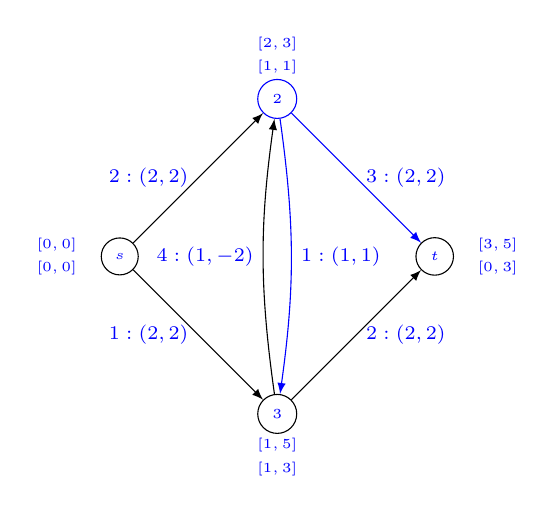
\begin{tikzpicture}[font=\tiny]
        %nodes
        \node at (-0.8, 0.15) {\blue{$[0,0]$}};
        \node at (-0.8, -0.15) {\blue{$[0,0]$}};
        \node[circle, draw] (s) at (0, 0) {\blue{$s$}};
        \node at (2, 2.7) {\blue{$[2, 3]$}};
        \node at (2, 2.4) {\blue{$[1, 1]$}};
        \node[blue, circle, draw] (a) at (2, 2) {\blue{$2$}};
        \node at (2, -2.4) {\blue{$[1, 5]$}};
        \node at (2, -2.7) {\blue{$[1, 3]$}};
        \node[circle, draw] (b) at (2, -2) {\blue{$3$}};
        \node at (4.8, 0.15) {\blue{$[3, 5]$}};
        \node at (4.8, -0.15) {\blue{$[0, 3]$}};
        \node[circle, draw] (t) at (4, 0) {\blue{$t$}};
        %edges
        \path [draw,-latex] (s) to node[left]{\scriptsize\blue{$2: (2, 2)$}} (a);
        \path [draw,-latex] (s) to node[left]{\scriptsize\blue{$1: (2, 2)$}} (b);
        \path [blue, draw,-latex] (a) to node[right]{\scriptsize\blue{$3: (2, 2)$}} (t);
        \path [draw,-latex] (b) to node[right]{\scriptsize\blue{$2: (2, 2)$}} (t);
        \path [blue, draw,-latex] (a) edge [bend left=8] node[right]{\scriptsize\blue{$1: (1, 1)$}} (b);
        \path [draw,-latex] (b) edge [bend left=8] node[left]{\scriptsize\blue{$4: (1, -2)$}} (a);
      \end{tikzpicture}
      \caption{Arcs explored the for loop at line \ref{algo1:setp:explore_arcs} when \blue{$i = 2$}.}
    \end{figure}
  \end{multicols}
\end{frame}


\begin{frame}
  \frametitle{Algorithm}
  \framesubtitle{Example}
  \begin{multicols}{2}
    State at the end of \blue{$4$}th iteration of the while at line \ref{algo1:setp:main_while}:
    \begin{itemize}   
      \item \blue{$\Lambda_s = \{ ((0, 0, 1, 1, 0, 0, 0), 0) \}$};
      \item \blue{$\Lambda_2 = \{((3, 0, 3, 1, 1, 1, 0), 5)\}$};
      \item \blue{$\Lambda_3 = \{((2, 2, 2, 1, 0, 1, 0), 1)\}$};
      \item \blue{$\Lambda_t = \{((5, 2, 4, 1, 1, 1, 1), 8)\}$};
      \item \blue{$N = \emptyset$};
    \end{itemize}   
    \begin{figure}[H]
      \centering
      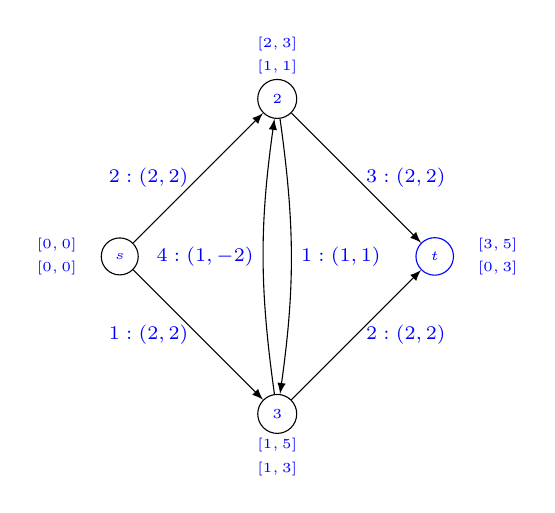
\begin{tikzpicture}[font=\tiny]
        %nodes
        \node at (-0.8, 0.15) {\blue{$[0,0]$}};
        \node at (-0.8, -0.15) {\blue{$[0,0]$}};
        \node[circle, draw] (s) at (0, 0) {\blue{$s$}};
        \node at (2, 2.7) {\blue{$[2, 3]$}};
        \node at (2, 2.4) {\blue{$[1, 1]$}};
        \node[circle, draw] (a) at (2, 2) {\blue{$2$}};
        \node at (2, -2.4) {\blue{$[1, 5]$}};
        \node at (2, -2.7) {\blue{$[1, 3]$}};
        \node[circle, draw] (b) at (2, -2) {\blue{$3$}};
        \node at (4.8, 0.15) {\blue{$[3, 5]$}};
        \node at (4.8, -0.15) {\blue{$[0, 3]$}};
        \node[blue, circle, draw] (t) at (4, 0) {\blue{$t$}};
        %edges
        \path [draw,-latex] (s) to node[left]{\scriptsize\blue{$2: (2, 2)$}} (a);
        \path [draw,-latex] (s) to node[left]{\scriptsize\blue{$1: (2, 2)$}} (b);
        \path [draw,-latex] (a) to node[right]{\scriptsize\blue{$3: (2, 2)$}} (t);
        \path [draw,-latex] (b) to node[right]{\scriptsize\blue{$2: (2, 2)$}} (t);
        \path [draw,-latex] (a) edge [bend left=8] node[right]{\scriptsize\blue{$1: (1, 1)$}} (b);
        \path [draw,-latex] (b) edge [bend left=8] node[left]{\scriptsize\blue{$4: (1, -2)$}} (a);
      \end{tikzpicture}
      \caption{Arcs explored the for loop at line \ref{algo1:setp:explore_arcs} when \blue{$i = t$}.}
    \end{figure}
  \end{multicols}
\end{frame}


\begin{frame}
\printbibliography
\end{frame}

\end{document}
